\documentclass[12pt]{article}

\usepackage[margin=1in]{geometry}
\usepackage{graphicx}
\usepackage{amsmath}
\usepackage{adjustbox}

\begin{document}
	\begin{titlepage}
		\begin{center}
			\hspace{0pt}
				\vfill
					\Huge CS 355: Program 2\\
					\Large Josh Patton \& Vaishak Menon\\
					\Large 04/03/2023
				\vfill
			\hspace{0pt}
            \small We declare that we have completed this assignment in accordance with 
            the UAB Academic Integrity Code and the UAB CS Honor Code. We have 
            read the UAB Academic Integrity Code and understand that any breach 
            of the Code may result in severe penalties.
            We  also  declare  that  the  following  percentage  distribution 
            faithfully  represents  individual  group  members’  contributions  to 
            the completion of the assignment\\
            \small Vaishak Menon, 50\% contribution, Partial Code Work and Partial Report Work, VM, 04/03/2023
            \small Josh Patton, 50\% contribution, Partial Code Work and Partial Report Work, JP, 04/03/2023
		\end{center}
	\end{titlepage}
	\newpage
	\begin{center}
	\Large Report\\
	\end{center}
    \begin{enumerate}
        \item Functionality:
        \subitem The code has 3 main functions: shuffleDecks, calculateCorrelations, and plotR. The calculateCorrelations function 
        will create an array of size n based on the given bounds. It will then call shuffleDecks to get the properly shuffled array 
        and then compute the correlation coefficient on every shuffle done. After the shuffling is complete, we call plotR to 
        plot the correlation for each run.
    \end{enumerate}
    \begin{center}
        \small First Run
    \end{center}
    \begin{enumerate}
        \item Plot r with respect to the times of shuffling. After how many shuffles are the cards 
        in the most random order? (That is, when is r at a minimum value?)
        \subitem The cards are in the most random order at shuffle 5 and 10\\
        \begin{minipage}[t]{\linewidth}
            \centering
            \adjustbox{valign=t halign=t}
            {
              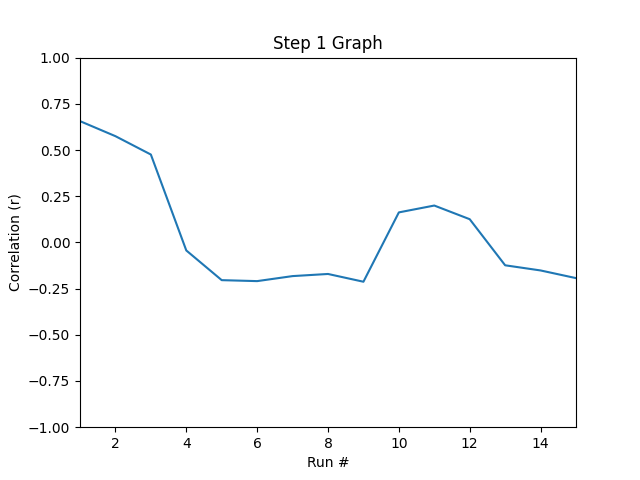
\includegraphics[width=.7\linewidth]{Figure_1.png}
            }
            \medskip       
        \end{minipage}
        \item Do the cards return to their original order?  After how many runs?
        \subitem Based on the correlations we collected, the cards do not return to the original order.
        \item Is a total of 15 runs enough to return to the original order?
        \subitem 15 runs were not enough to return to the original order.
        \item If not, does it appear that the cards will return to their original order in a relatively 
        small number of shuffles?
        \subitem It does not currently look like it will return, 
                 but there is the possiblity of them returning to the same order over a larger number of shuffles.
    \end{enumerate}
    \newpage
    \begin{center}
        \small Second Run
    \end{center}
    \begin{enumerate}
        \item Plot r with respect to the times of shuffling. After how many shuffles are the cards 
        in the most random order? (That is, when is r at a minimum value?)
        \subitem The cards are in the most random order at shuffle 8, which is the lowest point for this graph.\\
        \begin{minipage}[t]{\linewidth}
            \centering
            \adjustbox{valign=t halign=t}
            {
              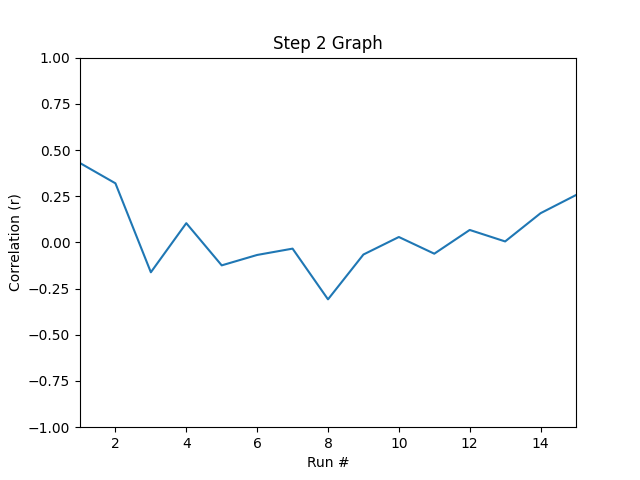
\includegraphics[width=.7\linewidth]{Figure_2.png}
            }
            \medskip       
        \end{minipage}
        \item Do the cards return to their original order?  After how many runs?
        \subitem Based on the correlations we collected, the cards do not return to the original order.
        \item Is a total of 15 runs enough to return to the original order?
        \subitem 15 runs were not enough to return to the original order.
        \item If not, does it appear that the cards will return to their original order in a relatively 
        small number of shuffles?
        \subitem For this specific test case, it looks like the order is rebounding back to the original, 
                 there may be a chance that it goes back, but this would require more testing.
    \end{enumerate}
    \newpage
    \begin{center}
        \small Third Run
    \end{center}
    \begin{enumerate}
        \item Plot r with respect to the times of shuffling. After how many shuffles are the cards 
        in the most random order? (That is, when is r at a minimum value?)
        \subitem The cards are in the most random order at shuffle 10, which is the lowest point for this graph.\\
        \begin{minipage}[t]{\linewidth}
            \centering
            \adjustbox{valign=t halign=t}
            {
              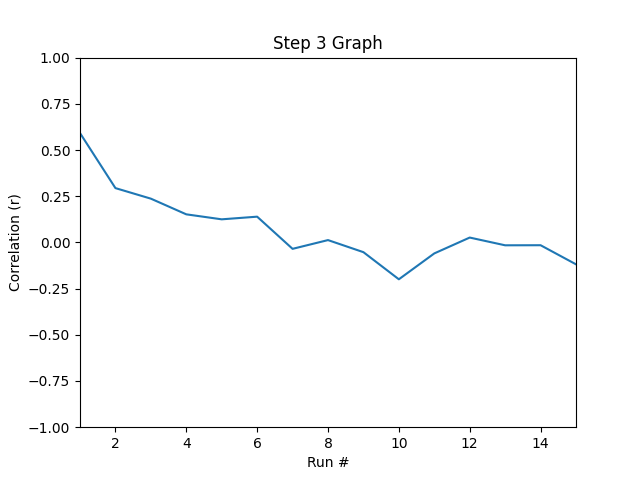
\includegraphics[width=.7\linewidth]{Figure_3.png}
            }
            \medskip       
        \end{minipage}
        \item Do the cards return to their original order?  After how many runs?
        \subitem Based on the correlations we collected, the cards do not return to the original order.
        \item Is a total of 15 runs enough to return to the original order?
        \subitem It is not enough to get back to the original order within 15 runs.
        \item If not, does it appear that the cards will return to their original order in a relatively 
        small number of shuffles?
        \subitem It does not currently look like it will return, 
                 but there is the possiblity of them returning to the same order over a larger number of shuffles.
    \end{enumerate}
    \newpage
    \begin{center}
        \small Fourth Run
    \end{center}
    \begin{enumerate}
        \item Plot r with respect to the times of shuffling. After how many shuffles are the cards 
        in the most random order? (That is, when is r at a minimum value?)
        \subitem The cards are in the most random order at shuffle 8 or 9, which is the lowest point for this graph.\\
        \begin{minipage}[t]{\linewidth}
            \centering
            \adjustbox{valign=t halign=t}
            {
              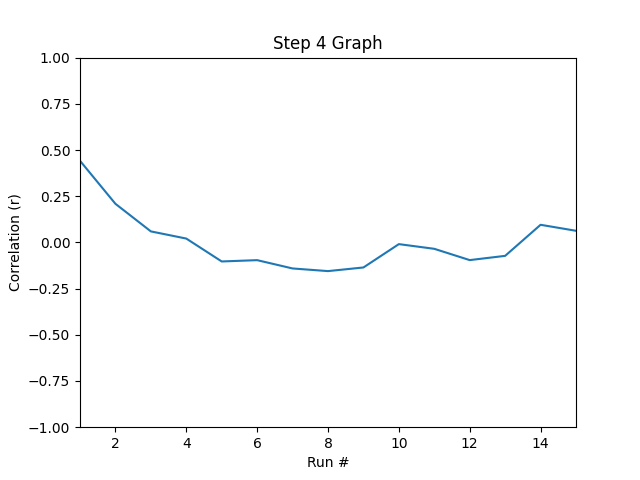
\includegraphics[width=.7\linewidth]{Figure_4.png}
            }
            \medskip       
        \end{minipage}
        \item Do the cards return to their original order?  After how many runs?
        \subitem Based on the correlations we collected, the cards do not return to the original order.
        \item Is a total of 15 runs enough to return to the original order?
        \subitem It does not reach the original order within 15 runs.
        \item If not, does it appear that the cards will return to their original order in a relatively 
        small number of shuffles?
        \subitem Based on the graph, it does not seem probable that the order will return to the 
                 original order, but without testing many more cases it will not be possible to tell.
    \end{enumerate}
\end{document}